\section{Methods and materials}
\label{sec:methods}

\subsection{Specimens and physical models}
I used a single \SI{6}{\year} old specimen (\fref{fig:methods:specimens}A) of \Citrusxparadisi\ (grapefruit) for all measurements. This specimen was germinated in Toledo, Ohio in January of 2014. As it grew, it spent its summers in the bright outdoors and winters in the relatively dark indoors, staying in a plastic pot throughout its life. This caused it to grow top heavy, with larger leaves in the canopy and smaller leaves in its understory. Additionally, it was subject to attacks from tetranychid mites each winter, leaving many leaves scarred. At the time of these trials, the specimen had just ended its winter indoor period, causing it to experience rapid growth. It stood at \SI{1.04}{\meter} tall and measured \SI{0.635}{\meter} across at its widest point; drag measurements focused on the plant's disproportionately large top.

To remove the effects of flexibility, I also created a physical model (\fref{fig:methods:specimens}C) of a single \Cxparadisi\ leaf using \SI{0.1}{\milli\meter} thick aluminum sheeting from a food container (Chipotle; 6658 Airport Hwy, Holland, OH). To prepare the physical model, I traced an actual leaf and cut the profile of the model to match. The physical model was mounted on a wooden pencil to provide a rigid attachment point compared to the typical flexible leaf petioles on \Cxparadisi. 
\begin{figure}
\begin{center}
%\includegraphics[width=0.3\columnwidth]{figures/FullPlant.jpg}
%\includegraphics[width=0.3\columnwidth]{figures/SingleLeaf.jpg}
%\includegraphics[width=0.3\columnwidth]{figures/MeasuredModel.jpg}
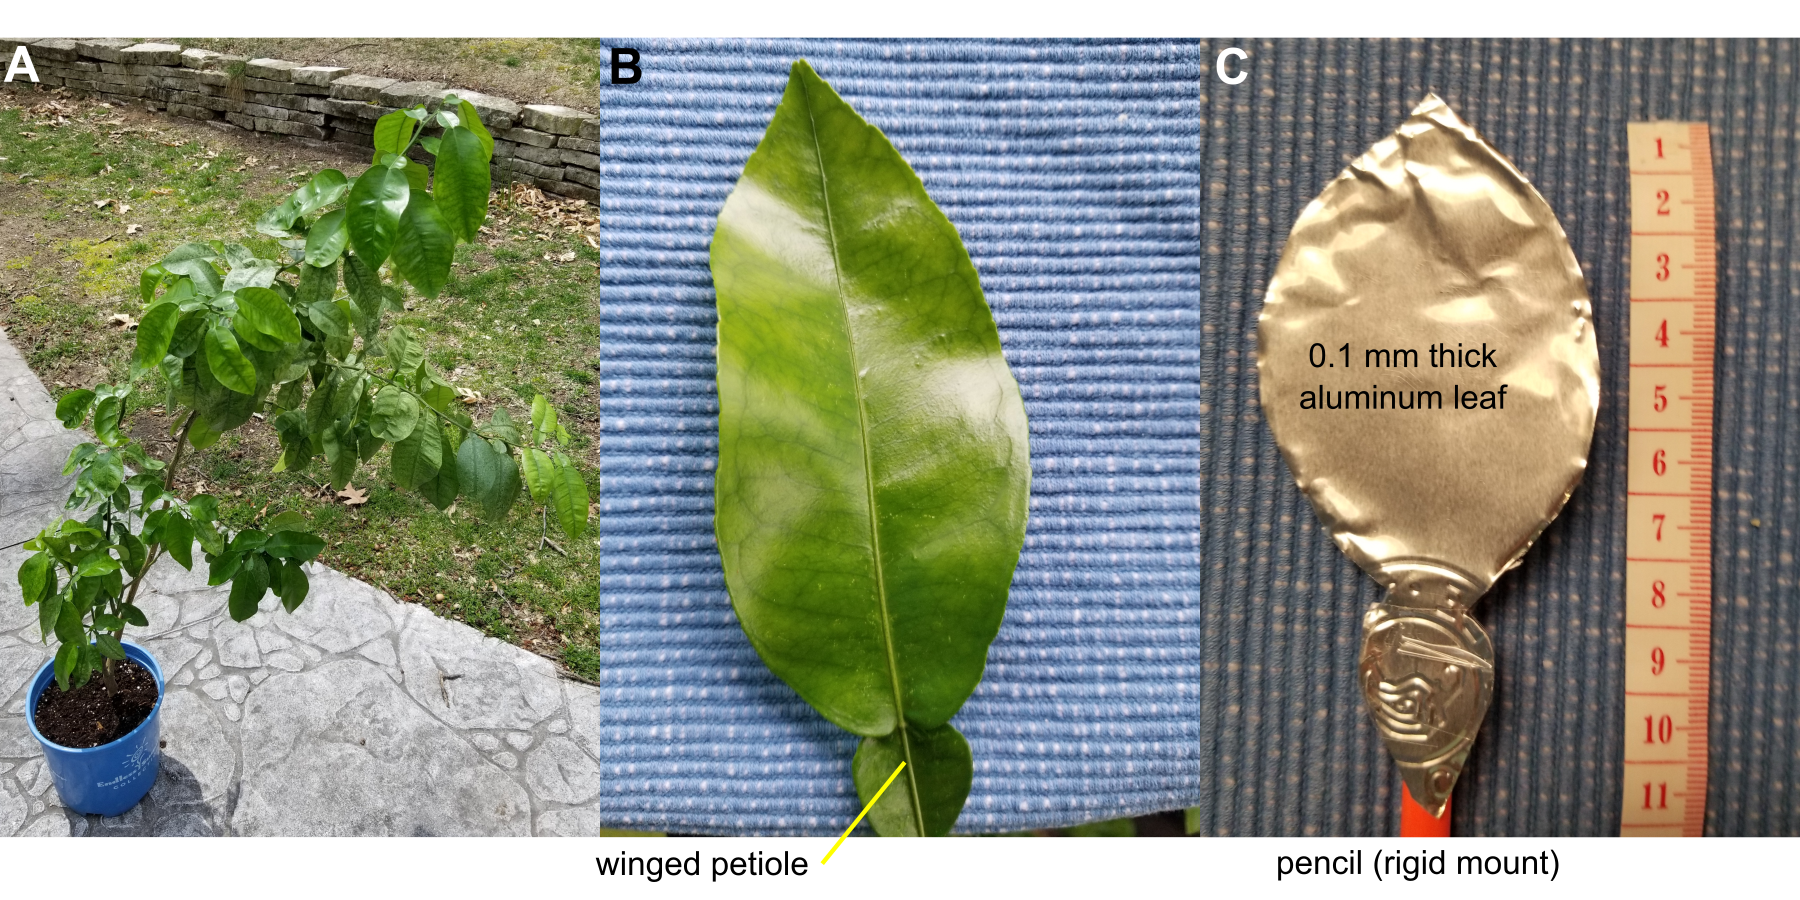
\includegraphics[width=6in]{figures/fig1.png}
\end{center}
\caption{(A) Specimen of \Citrusxparadisi\ (grapefruit), height \SI{1}{\meter}; (B) single grapefruit leaf showing winged petiole; and (C) rigid physical model of a single grapefruit leaf.}
\label{fig:methods:specimens}
\end{figure}








\subsection{Area measurements}
Because air was blowing from relatively close to the plant, only the area which was directly in front of the fan opening would be exposed to wind. The plant was of a complex shape; to obtain measurements of area normal to the flow ($A$ in \fref{eq:drag}), I used scale-calibrated images and color blob detection/segmentation in \Matlab\ (Mathworks; Natick, MA) (\fref{fig:methods:area}A). Images were taken with the same smartphone camera at a long enough distance to avoid foreshortening and lens distortion; images with and without the plant/leaf were taken from the same location. I took a reference image, without the specimen, with the fan aperture covered with a piece of black construction paper. I then took a similar image with the \Cxparadisi\ specimen present, and used the \Matlab\ \lstinline{colorThresholder} routine to obtain the proportion of area of the fan aperture covered by the specimen. This was then multiplied by the known area of the fan aperture to find the area of the \Cxparadisi\ specimen normal to flow. Identical methods were used to obtain the area of the rigid physical model of a single grapefruit leaf (\fref{fig:methods:area}B). Additional details on the image processing methods are provided in \fref{sec:A}. 
\begin{figure}
\begin{center}
%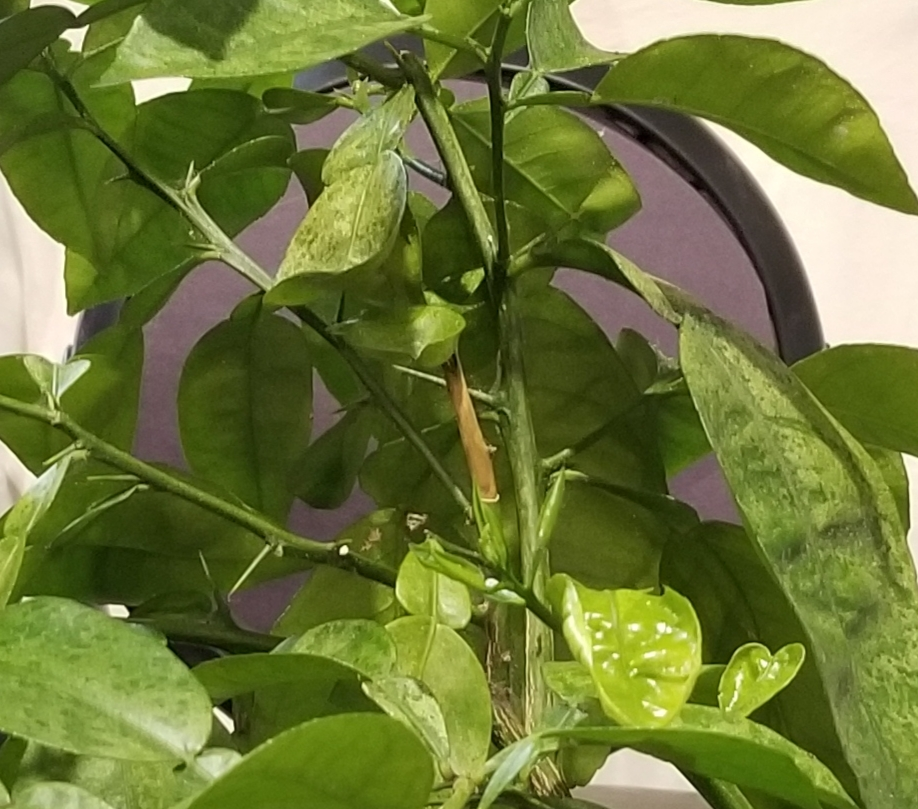
\includegraphics[width=0.3\columnwidth]{figures/Fan.jpg}
%\includegraphics[width=0.3\columnwidth]{figures/MetalLeaf.jpg}
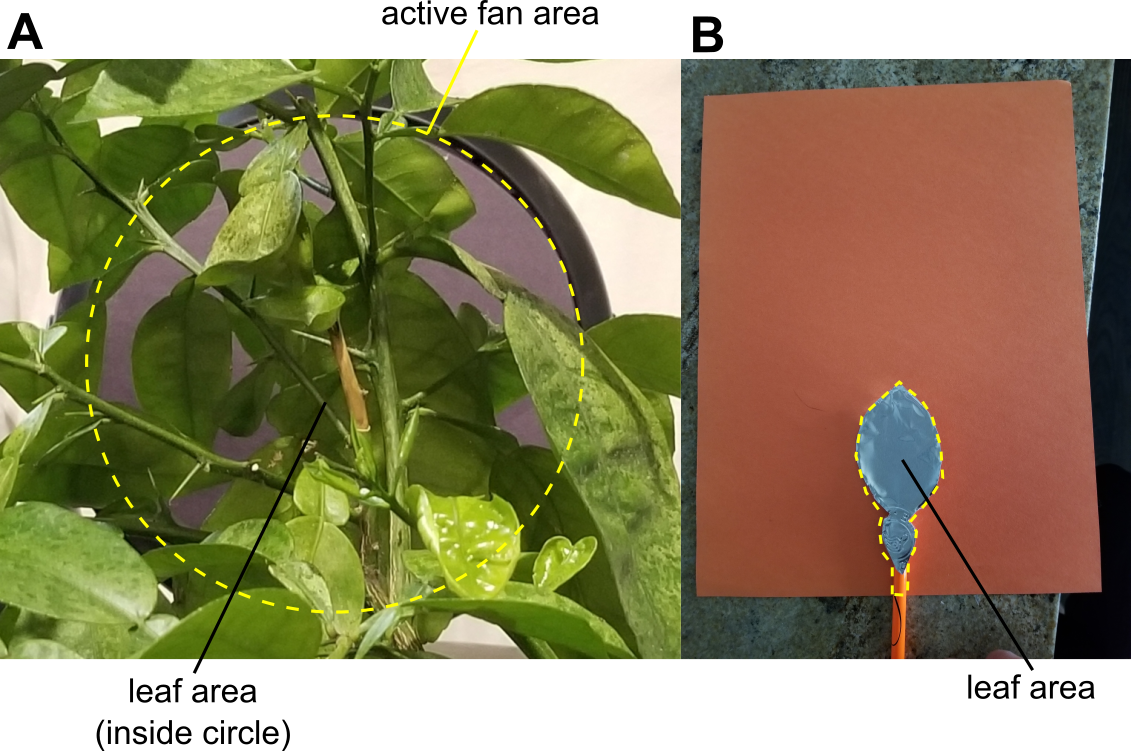
\includegraphics{figures/fig2.png}
\end{center}
\caption{Area measurements on (A) \Cxparadisi\ specimen and (B) rigid physical model of a single grapefruit leaf.}
\label{fig:methods:area}
\end{figure}





\subsection{Drag measurements}
Because of the COVID-19 pandemic, I did not have access to force instrumentation in lab; instead I used an elastic cord of a known spring constant and measured its displacement when attached to the specimens under a wind load. The cord (\SI{2}{\milli\meter} diameter) was obtained from a party mask. 

To measure drag, I attached the cord between a heavy, stationary chair and the specimens, as shown in \fref{fig:methods:drag}. The elastic cord was connected to a stiff rope (\SI{5}{\milli\meter} diameter, nylon), which was then tied off to the plant using a short, thick pipe cleaner wrapped around the main stem. Flow was provided by a 15-inch (\SI{0.38}{\meter}) fan ( HT-908 Turbo Force Room Air Circulator; Honeywell; Charlotte, NC) on a separate, stationary base \SI{1}{\meter} away. A ruler was used to judge the linear displacement of the elastic cord in the direction of flow.  Before drag measurements with specimens, the spring constant $K$ of the elastic cord (including rope and pipe cleaners) was found to be \SI{103}{\newton\per\meter} (\SI{0.059}{\poundforce\per\inch}) by hanging a known \SI{1.214}{\pound} (\SI{0.55}{\kilo\gram}) mass and measuring the resulting \SI{20.6}{\inch} (\SI{0.523}{\meter}) displacement. The spring constant $K$ provided a way to calculate $D$ in \fref{eq:drag} from the observed displacement. Drag was measured five times at each of the fan's three speed settings. A slow motion video of the plant's leaves was taken at the highest fan setting using a smartphone camera (Galaxy S8; Samsung; Seoul, South Korea) operated at \SI{240}{\frame\per\second}. Zoomed slow motion video was also used to aid in reading the deflection for the rigid physical model of a single leaf, which was markedly smaller than deflections observed in the whole plant specimen. 

Normally, air velocity measurements would be taken along with drag measurements to allow computation of a drag coefficient ($C_D$ in \fref{eq:drag}) as well as $\operatorname{Re}$. However, this was not possible due to COVID-19; therefore the results are left in terms of drag force ($D$) and the ratio of drag/area ($D/A$). 

% Fig 1 is good but cluttered, can we zoom in on only the business part; or turn it into a drawing. Altnatively, add callouts and scale bar? Is there a shot more from the side, that shows the experimental rig without foreshortening? 
% Agreed, I'll put in a drawing instead to make it neater
\begin{figure}
\begin{center}
%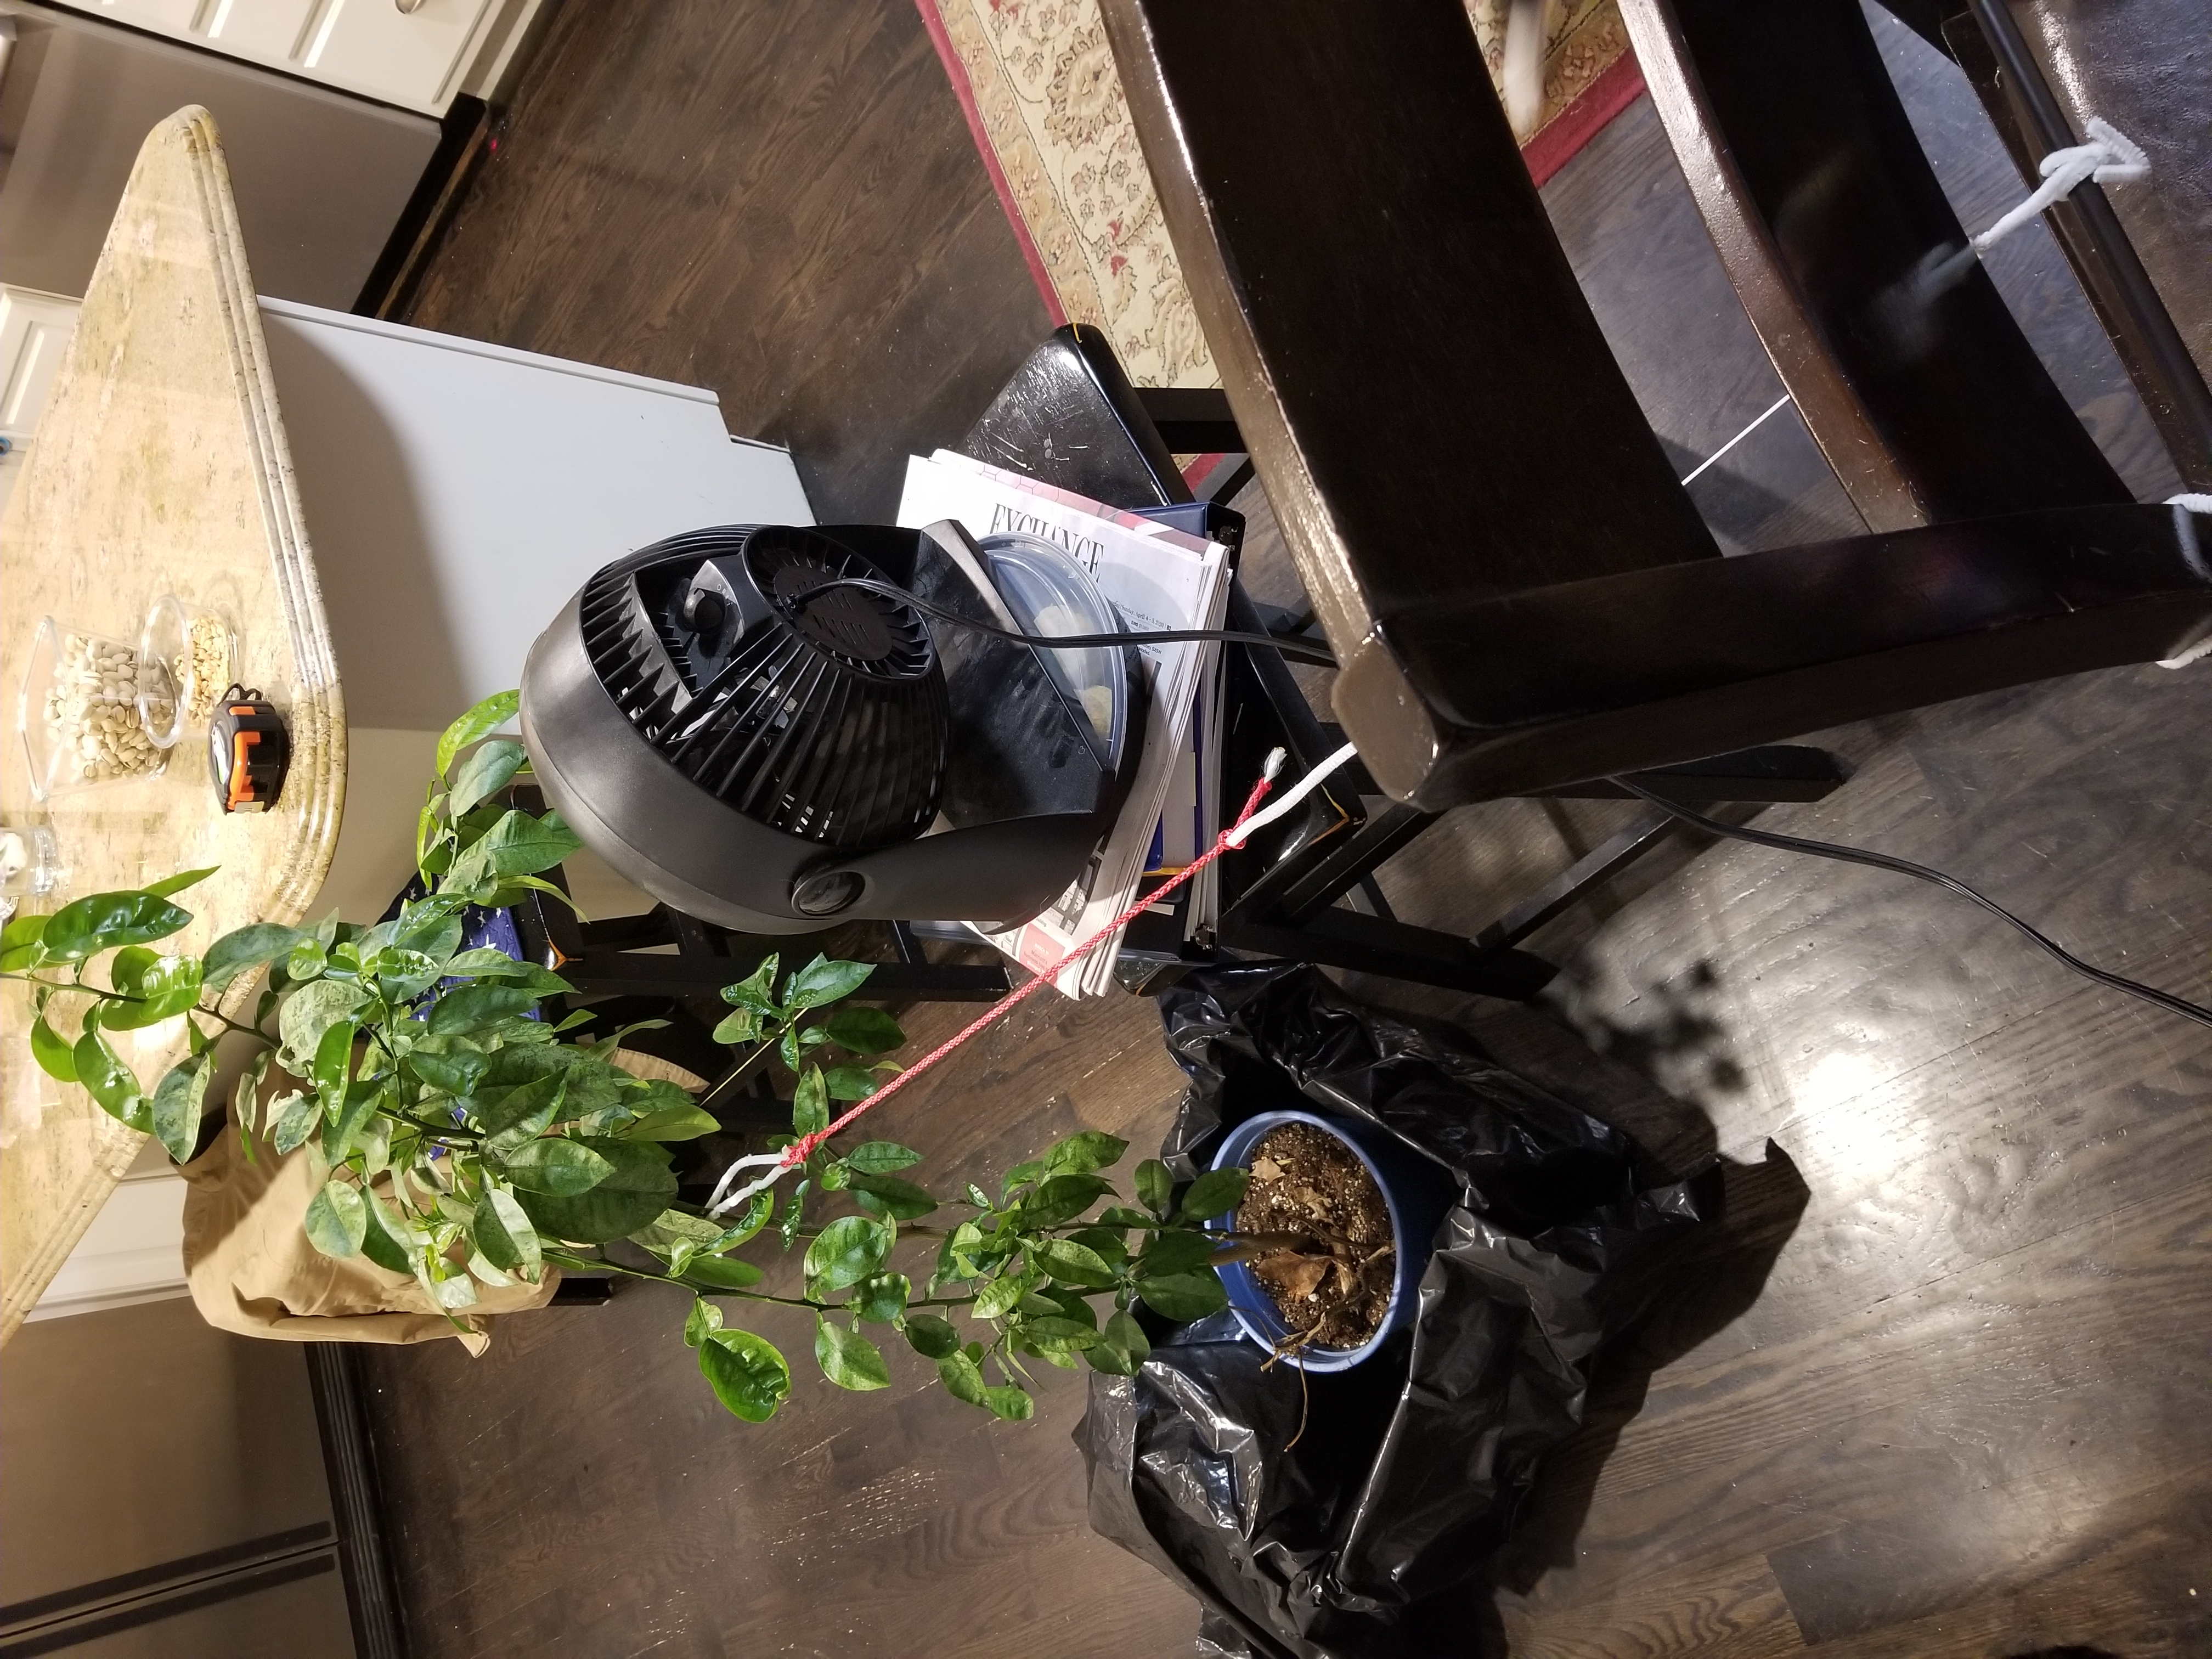
\includegraphics[width=0.18\columnwidth]{figures/Grapefruit_Setup.jpg} % ROTATE?!
%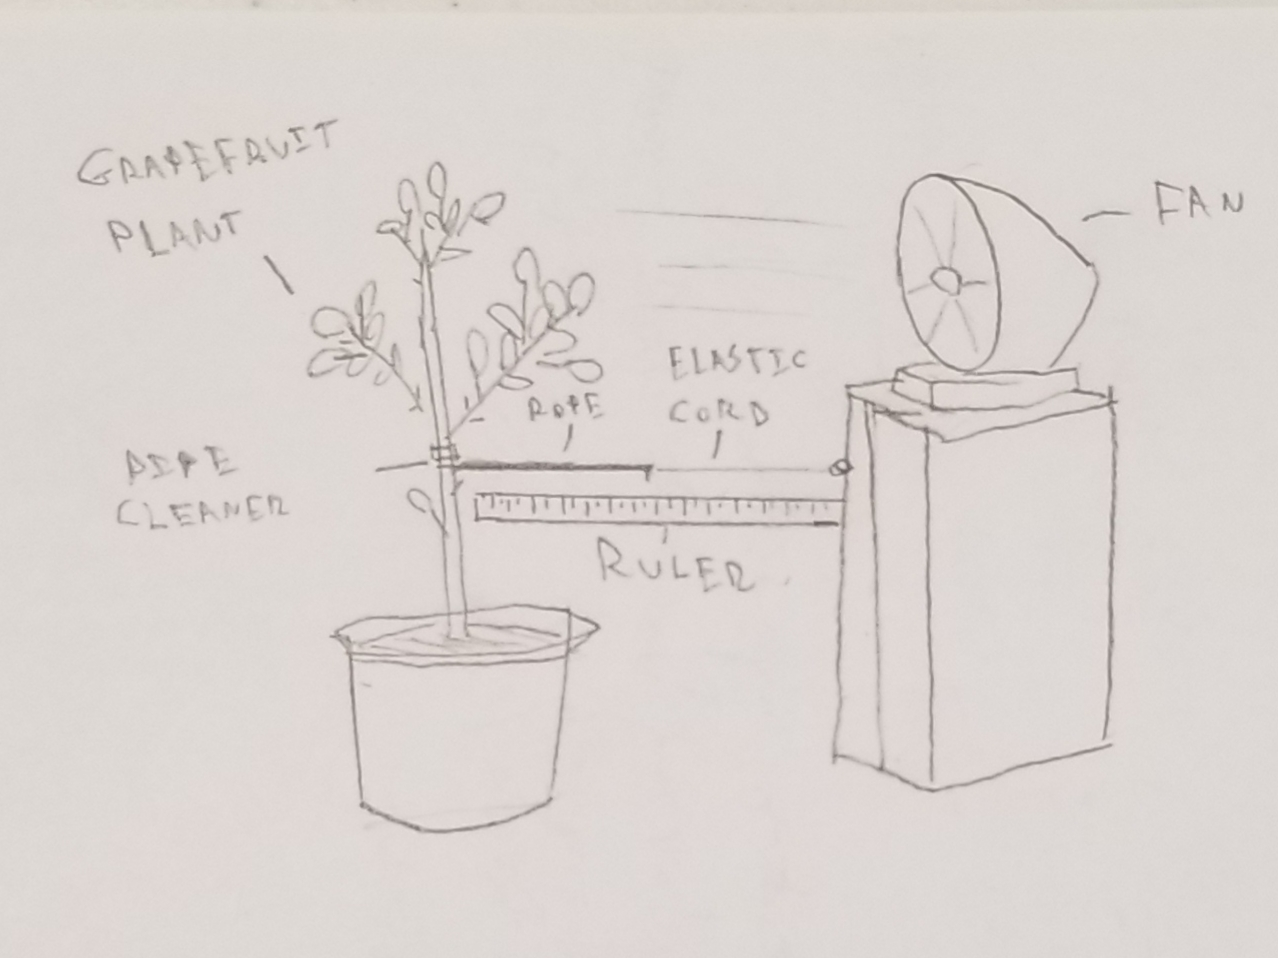
\includegraphics[width=0.4\columnwidth]{figures/Setup1.jpg} 
%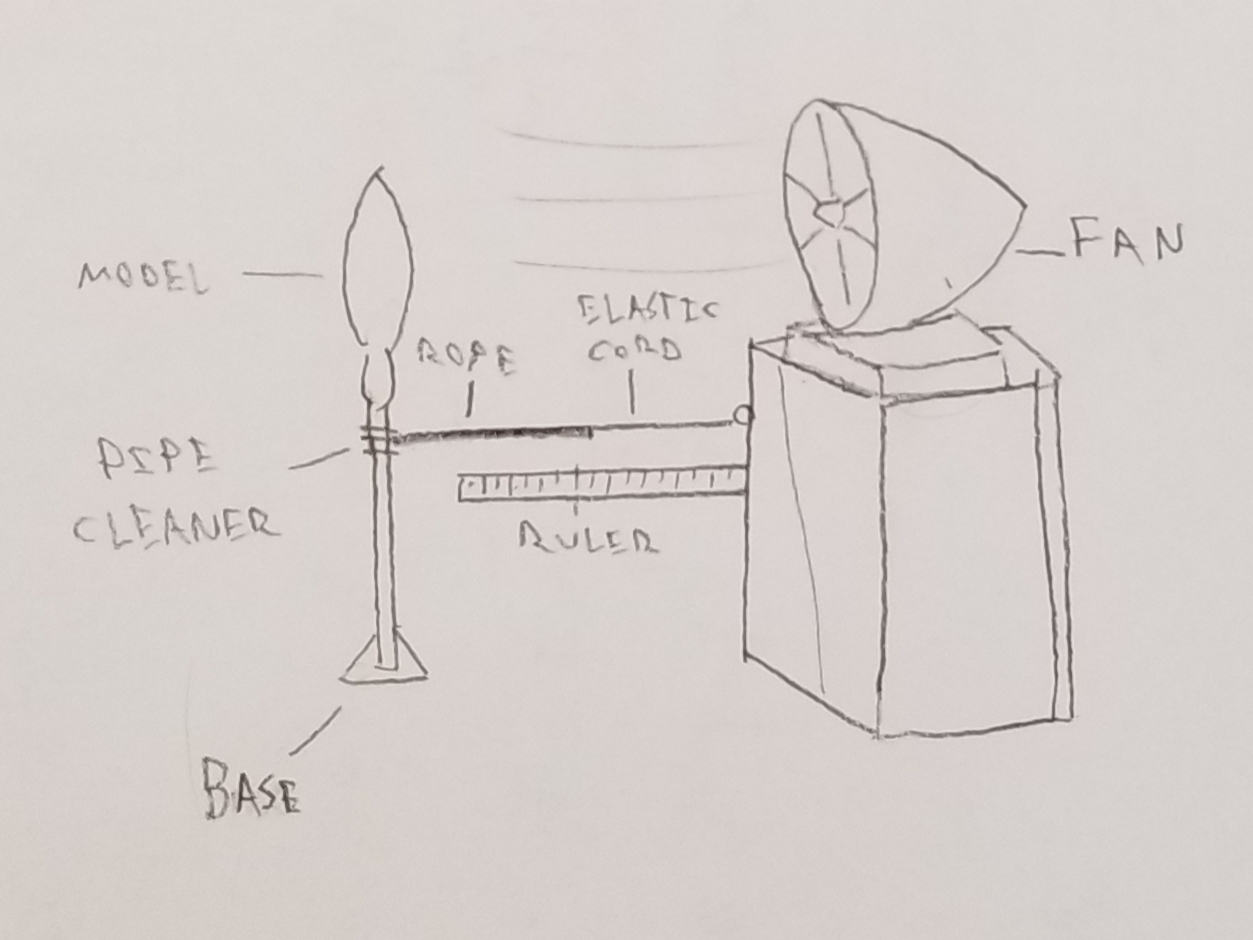
\includegraphics[width=0.4\columnwidth]{figures/Setup2.jpg}
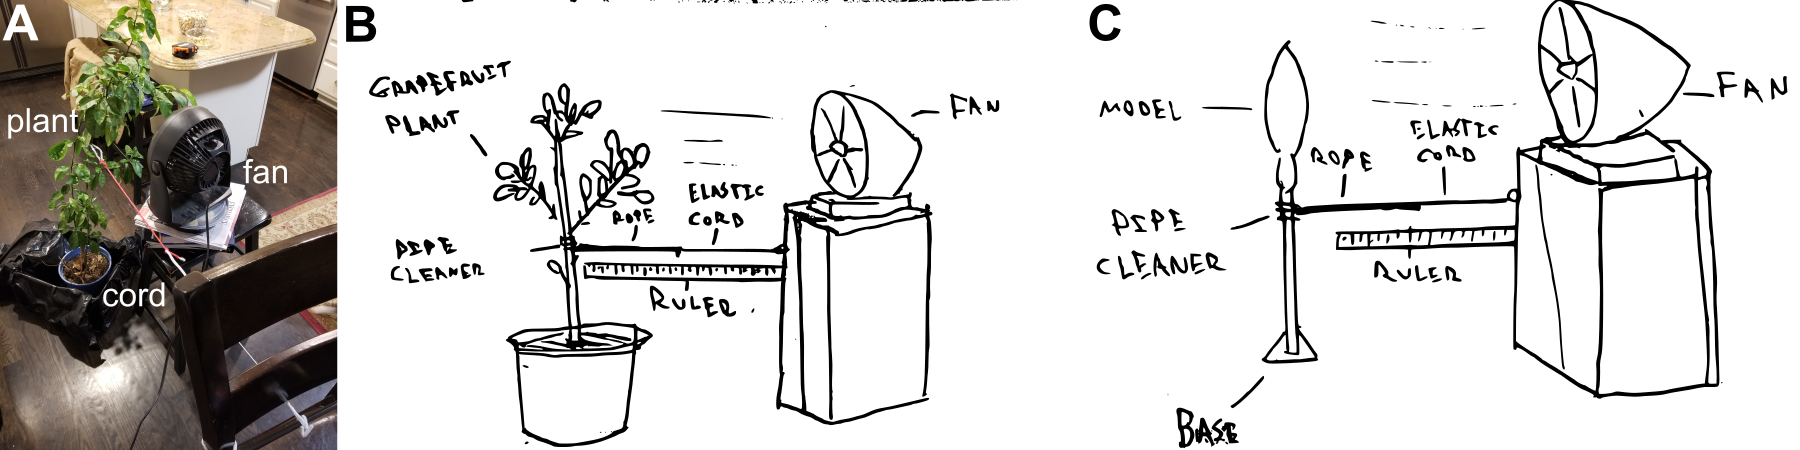
\includegraphics{figures/fig3.png}
\end{center}
\caption{Experimental setup to measure deflection and drag on (A, B) a live \Cxparadisi\ grapefruit plant; and (C) rigid physical model of a single grapefruit leaf.}
\label{fig:methods:drag}
\end{figure}













\subsection{Statistical analyses}
Statistical analyses of the effects of both leaf and fan speed on drag ($D$) and drag/area ($D/A$) were performed using R \citep{r2020} using two-way analysis of variance (ANOVA); plots were prepared using the \lstinline{tidyverse} and \lstinline{ggplot2} libraries \citep{wickham2019tidyverse}.

%Applying the percent difference formula
%\[D=100*\frac{2*|V1-V2|}{|V1-V2|}\]
%yields a difference of 17 percent between the drag to area ratios of the model and the actual plant at fan setting 3. 
% First - this is a result (17%) so belongs in results
% Also - the percent difference formula here doesn't quite make sense? 
















